\documentclass[11pt]{article}

\usepackage{changepage}
\usepackage{amsmath}
\usepackage{amsfonts}
\usepackage{xfrac}
\usepackage{faktor}
\usepackage{enumitem}
\usepackage[a4paper, total={7.25in, 10in}]{geometry}
\usepackage{url}
\usepackage{indentfirst}
\usepackage{hanging}
\usepackage[document]{ragged2e}
\usepackage[notes, short, backend=biber]{biblatex-chicago}
\usepackage{cmsendnotes}
\usepackage{hyperref}
\usepackage[rgb]{xcolor}
\usepackage{tikz}
\usepackage{pgfplots}

\ifdefined\HCode
   \def\pgfsysdriver{pgfsys-dvisvgm4ht.def}
\fi

\addbibresource{5-gorenstein-and-non-gorenstein-singularities.bib}
\setlength{\parindent}{0pt}
\setlength{\RaggedRightParindent}{0pt}
\setlength{\parskip}{1em}

\newcommand{\BExcerpt}{}
\newcommand{\EExcerpt}{}

\newcommand{\Question}{\noindent\textbf{Question.}~}

\definecolor{o0}{HTML}{888888}
\definecolor{o1}{HTML}{f43753}
\definecolor{o2}{HTML}{b3deef}
\definecolor{o3}{HTML}{ffc24b}
\definecolor{o4}{HTML}{73cef4}
\definecolor{o5}{HTML}{d3b987}
\definecolor{o6}{HTML}{c9d05c}
\definecolor{o7}{HTML}{f47192}

\DeclareMathOperator{\depth}{depth}
\DeclareMathOperator{\Spec}{Spec}
\DeclareMathOperator{\Hom}{Hom}
\DeclareMathOperator{\Ext}{Ext}

\pgfplotsset{compat=1.18, every axis/.append style={xmin=-2, ymin=-2, xmax=2, ymax=2, smooth, samples=100, axis lines=center}, view/h=20, axis line style={o0}, every tick label/.append style={font=\tiny}, every axis legend/.append style={draw=none, font=\small}}

\title{Gorenstein and Non-Gorenstein Singularities}
\date{5 June 2025}

\begin{document}
    \maketitle
    {\itshape\BExcerpt This is a student seminar talk I gave back in December, mostly to try and understand the correspondence between classes of not-quite-regular rings and the singularities of their spectra.\EExcerpt It was shamefully written pretty much just for myself, but I did also mislead some of my analyst friends into attending, so I was trying to be more fun and casual than technical. Since then, I've both passed my quals and lost the original notes I wrote for this talk, so I really need you to trust me that it was better at the time.}

    In commutative algebra, we have an idea of how ``nice'' a local ring might be -- in ascending order, the usual list starts with Cohen-Macaulay rings, then Gorenstein rings, then complete intersection rings, then regular local rings. Recalling the definitions, a local ring \((A, \mathfrak{m}, k)\) is Cohen-Macaulay if \(\dim A = \depth R\), and \(A\) is regular if \(\mathfrak{m}\) is generated by \(\dim A\) elements. \(A\) is a complete intersection if \(\overline{A}\) is the quotient of a regular local ring by an ideal \((\boldsymbol{x})\), where \(\boldsymbol{x}\) is a regular sequence. 
    
    The three kinds of ring we've defined so far have intuitive geometric interpretations as well. On a variety (over a perfect field, for technical reasons), the local ring at a point \(p\) is regular if and only if the variety is smooth, where you can imagine ``smooth'' meaning smooth in the analytic sense:

    \begin{tabular}{cc}
        \begin{tikzpicture}[baseline=(current bounding box.north)]
            \begin{axis}[zticklabels={}]
%                \node[font=\small] at (0,1,1) {\(\displaystyle X = \Spec \sfrac{k[x,y]}{\left(y^2-(x^3 + x)\right)}\)};
                \draw[clip] (-2,-2,0) -- (-2,2,0) -- (2, 2, 0) -- (2, -2, 0) -- cycle;
                \draw[fill=o3, fill opacity=0.15] (-2,-2,0) -- (-2,2,0) -- (2, 2, 0) -- (2, -2, 0) -- cycle;
                \addplot3[thick, contour gnuplot={draw color=o2, levels={0}, labels=false}] {y^2 - (x^3 + x)};
            \end{axis}
        \end{tikzpicture} & \begin{tikzpicture}[baseline=(current bounding box.north)]
            \begin{axis}[zticklabels={}]
 %               \node[font=\small] at (0,1,1) {\(\displaystyle Y = \Spec \sfrac{k[x,y]}{\left(y^2-x^3\right)}\)};
                \draw[clip] (-2,-2,0) -- (-2,2,0) -- (2, 2, 0) -- (2, -2, 0) -- cycle;
                \draw[fill=o3, fill opacity=0.15] (-2,-2,0) -- (-2,2,0) -- (2, 2, 0) -- (2, -2, 0) -- cycle;
                \addplot3[thick, contour gnuplot={draw color=o7, levels={0}, labels=false}] {y^2 - x^3};
            \end{axis}
        \end{tikzpicture}
    \end{tabular}

    Letting \(p = (0,0) \in \mathbb{A}^2\) be the point corresponding to \((x,y)\) in \(k[x,y]\), \(\mathcal{O}_{X,p}\) on the left is regular, but \(\mathcal{O}_{Y,p}\) on the right is not. Both are complete intersections, though, since their defining ideals are generated by one element and \(k[x,y]\) is a regular domain. I would say that \(Y\) has a complete intersection singularity at \(p\).

    \Question To understand the geometry encoded in Cohen-Macaulay rings, it's convenient that the Krull dimension of the ring matches the intuitive idea of dimension as a variety -- but what does the depth represent? 

    I've procrastinated in defining what a Gorenstein ring or a Gorenstein singularity is, so -- for a local ring \((A, \mathfrak{m}, k)\) of dimension \(n\), the following are equivalent:
    \begin{enumerate}[label=(\roman*)]
        \item \(A\) is \textit{Gorenstein};
        \item \(\operatorname{injdim} A < \infty\);
        \item \(\operatorname{injdim} A = n\);
        \item \(\Ext_A^i(k, A) = \delta_n^i k\);
        \item \(\Ext_A^i(k, A) = 0\) for some \(i > n\);
        \item \(A\) is Cohen-Macaulay and \(\Ext_A^n(k, A) = k\);
        \item \(A\) is isomorphic to its own canonical module \(\omega_A\).
    \end{enumerate}

    Geometrically, Gorenstein singularities are more mysterious. For example, the variety \(Y = \Spec \sfrac{k[x,y]}{(xy)}\) is Gorenstein (indeed, it is a complete intersection), but the variety \(X = \Spec \sfrac{k[x,y,z]}{\left(xy, xz, yz\right)}\) has a non-Gorenstein singularity at the origin:

    \begin{tabular}{cc}
        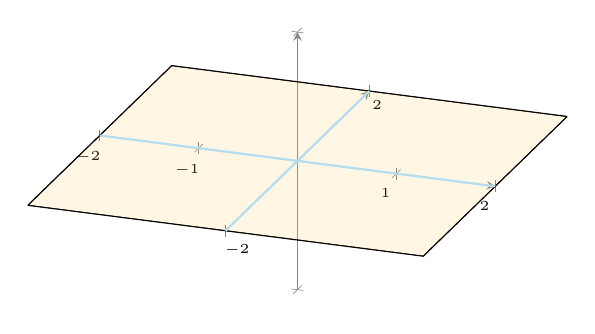
\begin{tikzpicture}[baseline=(current bounding box.north)]
            \begin{axis}[zticklabels={}]
  %              \node[font=\small] at (0,1,1) {\(\displaystyle Y = \Spec \sfrac{k[x,y]}{\left(xy\right)}\)};
                \draw[clip] (-2,-2,0) -- (-2,2,0) -- (2, 2, 0) -- (2, -2, 0) -- cycle;
                \draw[fill=o3, fill opacity=0.15] (-2,-2,0) -- (-2,2,0) -- (2, 2, 0) -- (2, -2, 0) -- cycle;
                \addplot3[thick, color=o2] table {
                    x y z
                    -2 0 0
                    2 0 0
                };
                \addplot3[thick, color=o2] table {
                    x y z
                    0 -2 0
                    0 2 0
                };
            \end{axis}
        \end{tikzpicture} & 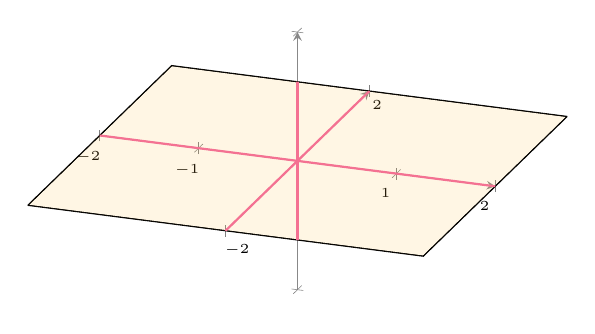
\begin{tikzpicture}[baseline=(current bounding box.north)]
            \begin{axis}[zticklabels={}]
   %             \node[font=\small] at (0,-2,-1) {\(\displaystyle X = \Spec \sfrac{k[x,y,z]}{\left(xy, xz, yz\right)}\)};
                \draw[clip] (-2,-2,0) -- (-2,2,0) -- (2, 2, 0) -- (2, -2, 0) -- cycle;
                \draw[fill=o3, fill opacity=0.15] (-2,-2,0) -- (-2,2,0) -- (2, 2, 0) -- (2, -2, 0) -- cycle;
                \addplot3[thick, color=o7] table {
                    x y z
                    -2 0 0
                    2 0 0
                };
                \addplot3[thick, color=o7] table {
                    x y z
                    0 -2 0
                    0 2 0
                };
                \addplot3[thick, color=o7] table {
                    x y z
                    0 0 -2
                    0 0 2
                };
            \end{axis}
        \end{tikzpicture}
    \end{tabular}

    Heuristically, we might expect this, but only because it's geometrically evident that \(X\) isn't a complete intersection -- \(X\) has codimension \(2\) but its defining ideal has \(3\) generators. To verify directly that \(X\) isn't Gorenstein is a little more laborious and, concerningly, attempting to verify criteria (iv) or (v) might require arbitrarily many computations. Instead, we can compute the canonical module of \(\mathcal{O}_{X,0}\) and determine that it is different than \(\mathcal{O}_{X,0}\) itself.

    Let \(R = k[x,y,z]\) -- first, we'll inspect the quotient map \(R \to \mathcal{O}_X \to 0\) and extend it to a free resolution \(F_\bullet\). We start with \[R^3 \xrightarrow{\begin{pmatrix}
    xy & yz & xz
    \end{pmatrix}} R \to \mathcal{O}_X \to 0.\] At the next iteration, we get \[F_\bullet: R^2 \xrightarrow{\begin{pmatrix}
        -z & 0\\
        y & -y\\
        0 & x
    \end{pmatrix}} R^3 \xrightarrow{\begin{pmatrix}
    xy & yz & xz
    \end{pmatrix}} R \to \mathcal{O}_X \to 0\]
    because if \(R^2\) is generated by \(\left\{e_1, e_2\right\}\), then \(\begin{pmatrix}
        -ze_1\\
        ye_1 -ye_2\\
        xe_2
    \end{pmatrix}\begin{pmatrix}
        xy & xz & yz
    \end{pmatrix} = 0\). This map has trivial kernel, so it completes our free resolution. Next, we apply \(\Hom(-,R)\) to obtain the dual resolution \[F^\bullet: 0 \to \mathcal{O}_X \to R \xrightarrow{d^0} R^3 \xrightarrow{d^1} R^2 \to 0\]

    This is an acyclic resolution of \(\mathcal{O}_X\) with respect to the functor \(\Hom(-,R)\), so \(\Ext^i(\mathcal{O}_X, R) = H^i(\Hom(F^\bullet, R))\). Now, \(R\) is a \(3\)-dimensional regular ring and \(\mathcal{O}_X\) is a \(1\)-dimensional \(R\)-algebra, so a theorem\autocite[\nopp 3.3.7]{BH98} tells us that \(\omega_{\mathcal{O}_{X,0}}\) is isomorphic to \(\Ext^2(\mathcal{O}_{X,0}, R_{(x,y,z)})\), which we now know is the cokernel of the map \(d^1\). For linear algebra reasons, \(d^1\) is the transpose of the map \(\begin{pmatrix}
        -z & 0\\
        y & -y\\
        0 & x
    \end{pmatrix}\) in the \(F_\bullet\) resolution. Since \(\mathcal{O}_X\) is the cokernel of \(\begin{pmatrix}
    xy & yz & xz
    \end{pmatrix}\), and these aren't the same, we've shown that \(\mathcal{O}_{X,0}\) isn't isomorphic to \(\omega_{\mathcal{O}_{X,0}}\), so \(\mathcal{O}_{X,0}\) isn't Gorenstein.

    There is an alternate way of showing that \(\mathcal{O}_{X,0}\) isn't Gorenstein that is more specific to this particular ring, but may be more illuminating combinatorially. Given a simplicial complex \(\Delta\) and a field \(k\), we can define a ring \(R\) to be the free commutative \(k\)-algebra generated by the vertex set of \(\Delta\), and an ideal \(I\) generated by the square-free monomials who \textit{don't} correspond to faces of the complex. The quotient \(\sfrac{R}{I}\) is called the \textit{Stanley-Reisner ring} of the complex. 
    
    It turns out that our coordinate ring \(\mathcal{O}_{X}\) is the Stanely-Reisner ring of a somewhat boring simplicial complex: 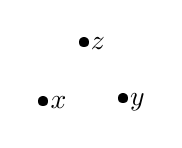
\begin{tikzpicture}[baseline=(current bounding box.center)]
        \node[] at (0,0) {\textbullet \(x\)};
        \node[] at (1, 0) {\textbullet \(y\)};
        \node[] at (0.5, 0.75) {\textbullet \(z\)};
    \end{tikzpicture} 

	Conveniently, we can detect if a Stanely-Reisner ring is Gorenstein (or Cohen-Macaulay) using only combinatorial data from the simplicial complex. 

    \Question What does it mean, ethically, for the coordinate ring of a variety to be Gorenstein?
    
    \textit{Eventually I will finish writing this and maybe even answer this question \(<3\)}
    \newpage
    \printbibliography[title={Bibliography}]
\end{document}
